\documentclass{article}
\usepackage{hyperref}
\usepackage{enumitem}
\usepackage{biblatex}
\usepackage{graphicx} 
\usepackage{amsmath}
\usepackage{float}
\usepackage[serbian]{babel}

% Title
\title{Klasifikacija malignog raka kože}
\author{
    Branko Grbić \\
    2/2020
    \and 
    Igor Zolotarev \\
    228/2019
}
\date{\today}

\usepackage[T1]{fontenc} % Add this line

\usepackage[margin=3cm]{geometry} % set 2cm margins

\addbibresource{your_bibliography_file.bib} % Specify your bibliography file here

\linespread{1.4}

\hypersetup{
    colorlinks=true,
    linkcolor=blue,
    filecolor=magenta,      
    urlcolor=cyan,
}


\begin{document}

\maketitle

% Abstract
%\begin{abstract}
%    ...
%\end{abstract}

\vfill
\hfill 
\section*{Fakultet}
Matematicki fakultet
\newline
Univerzitet u Beogradu

\section*{Mentor}
 Prof. Dr. Nenad Mitic
 \newline
Katedra za racunarstvo i informatiku

\newpage

\renewcommand{\contentsname}{Sadržaj}
\tableofcontents{}


\newpage
\section{Uvod} 
Melanoma je tip kancera kože, invazivna bolest uzrokovana abnormalnim rastom melanocitnih stanica u telu, koje imaju tendenciju da se repliciraju i šire kroz limfne čvorove kako bi uništile okolna tkiva [1]. Iako Melanoma obuhvata relativno mali procenat kancera kože, ubedljivo je najsmrtonosnija.
Nastaje u melanocitnim ćelijama koje proizvode melanin, pigment koji daje boju koži. Opasna priroda Melanome se ogleda u tome što ima mogućnost da se brzo rasprostrani na ostale delove tela, mnogo brže nego sve ostale varijante kancera kože.
Oštećene stanice razvijaju mladež na spoljnjem sloju kože, kategorizovan kao maligni ili benigni, dok se Melanom smatra kancerom, jer je opasniji i preteći po život. Ovaj kancer kože je globalno rasprostranjena i opasna bolest, sa 300.000 novih dijagnostikovanih slučajeva i preko 1 milion smrtnih slučajeva svakog meseca širom sveta u 2018. godini [2]. Melanom je postao široko rasprostranjen u svetu, postajući 19. najčešća bolest sa najvišom stopom smrtnosti. Zbog ovih stavki, od izuzetne je važnosti što pre identifikovati i sprečiti dalje širenje ove vrste kancera kože. Ovo predstavlja primarni motivator za konstrukciju modela za klasifikovanje kancera Melanome.
\par
Neke od osnovnih poteškoća koje se susreću pri identifikovanju Melanome mogu biti:

\begin{enumerate}
    \item \textbf {Složenost dijagnoze} - Melanome su vrsta malignih tumora kože koji se mogu razlikovati po svojoj morfologiji, boji, veličini i teksturi.
    \item \textbf {Varijabilnost u obliku i veličini} - Melanome mogu imati različite oblike, veličine i karakteristike koje se mogu razlikovati čak i unutar istog pacijenta.
    \item \textbf {Sličnosti sa benignim lezijama} - Ponekad melanomi mogu imati slične karakteristike kao i benigni madeži ili druge lezije na koži. Pronalaženje razlika između Melanoma i benignih lezija može praviti ozbiljne probleme i najiskusnijim dermatolozima.
    \item \textbf {Potreba za ranim otkrivanjem} - Melanoma ima potencijal da se širi i metastazira ako se ne dijagnosticira i leči na vreme. Stoga je važno da alati za otkrivanje budu što precizniji i brži kako bi se bolest otkrila u ranoj fazi.
\end{enumerate}

\par
Smisao ovog projekta leži u potrebi za klasifikacijom raka kože, radi brže i efikasnije detekcije. Inspiracija je bila postojeći rad na ovu temu koji pokazuje obećavajuće rezultate dubokim učenjem [3]. Korišćena su dva modela za mašinsko učenje trenirana na ISIC 2016 skupu podataka (podzadatak 3) [8]. Time, napravljen je rad koji poredi modele sa dubokim mašinskim učenjem (VGG) i modelom zasnovanim na drvetima odlučivanja (XGBoost).  

\section{Okruženje projekta}

\subsection{Jezik i neophodni moduli}
U ovom projektu koristi se Python 3 zbog njegove popularnosti u zajednici mašinskog učenja, bogatog skupa biblioteka i jednostavne sintakse [9]. Python omogućava brzu i efikasnu implementaciju algoritama mašinskog učenja i manipulaciju podacima. Sledeće biblioteke su korišćene:

\begin{itemize}
    \item \textbf{torch} - PyTorch je otvorena biblioteka za duboko učenje koja pruža fleksibilnost i efikasnost u implementaciji i treniranju neuralnih mreža.
    \item \textbf{torchvision} - Dodatak PyTorcha koji sadrži popularne modele, skupove podataka i transformacije za rad sa slikama.
    \item \textbf{numpy} - Biblioteka za rad sa nizovima i matricama, koja omogućava efikasne matematičke operacije potrebne za mašinsko učenje.
    \item \textbf{scikit-learn} - Biblioteka koja sadrži jednostavne i efikasne alate za rudarenje podacima (data mining) i analizu podataka, uključujući mnoge algoritme mašinskog učenja.
    \item \textbf{pickle} - Modul za serijalizaciju i deserializaciju objekata u Pythonu, što omogućava čuvanje i učitavanje modela mašinskog učenja.
    \item \textbf{matplotlib} - Biblioteka za kreiranje statičkih, animiranih i interaktivnih vizualizacija u Pythonu.
    \item \textbf{seaborn} - Biblioteka zasnovana na matplotlib-u koja omogućava jednostavno kreiranje atraktivnih i informativnih statističkih grafika.
    \item \textbf{pandas} - Biblioteka za manipulaciju i analizu podataka, koja pruža strukture podataka i operacije potrebne za rad sa tabelarnim podacima.
    \item \textbf{PIL} - Omogućava otvaranje i obradu različitih formata slika.
\end{itemize}

\subsection{Kako pokrenuti projekat}

Da biste pokrenuli repozitorijum, neophodno je pratiti sledeće korake:

\begin{enumerate}
    \item Preuzeti skup podataka.
    \item Instalirati Python 3 i njegove neophodne biblioteke.
    \item Podesiti argumente komandne linije (opciono).
    \item Koristeći Python, pokrenuti \texttt{main.py}.
\end{enumerate}

\textit{Za detaljnije instrukcije, posetiti repozitorijum i pročitati početnu README.md stranu [11]}

\section{Priprema podataka}
Priprema podataka u mašinskom učenju obuhvata sve korake i tehnike koje se primenjuju kako bi se sirovi podaci transformisali u format pogodan za analizu i treniranje modela. Ovaj ključni korak u procesu mašinskog učenja ima za cilj da obezbedi kvalitetne, relevantne i dobro strukturirane podatke koji će omogućiti efikasno učenje modela i generisanje tačnih predikcija. Priprema podataka podrazumeva niz aktivnosti, uključujući čišćenje podataka radi uklanjanja grešaka, nedostajućih vrednosti ili duplikata.

\begin{figure}[H]
    \centering
    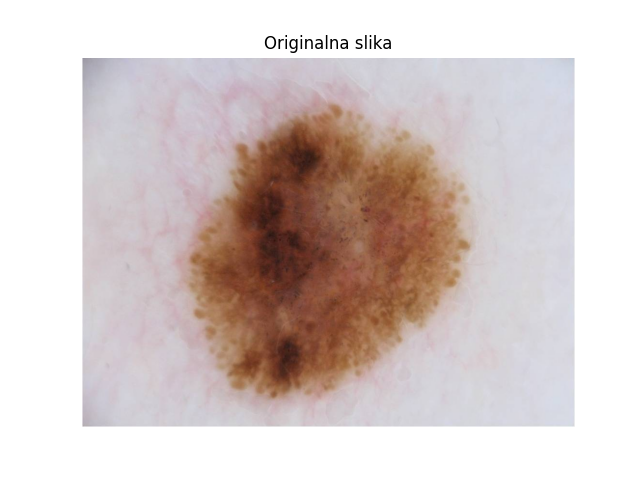
\includegraphics[width=0.4\textwidth]{slike_raka/original_image.png} 
    \caption{Prikaz instance skupa podataka - benigni tip raka kože} 
    \label{instanca skupa podataka}
\end{figure}

\subsection{Analiza skupa podataka}

Analiza skupa podataka pokazala je da imamo odvojene trening i test skupove. Trening skup se sastoji od 899 slika, od kojih je 726 označeno kao benigno, dok je 173 označeno kao maligno. Test skup sadrži 378 slika, od kojih je 303 benigno, a 75 maligno. Ovi podaci ukazuju na značajnu nebalansiranost klasa, što zahteva posebnu pažnju prilikom treniranja modela kako bi se osigurali tačni i nepristrasni rezultati.
\par
U skupu podataka nema nepostojećih vrednosti, što eliminiše potrebu za dodatnim čišćenjem podataka. Date slike su u JPEG formatu, ali različitih rezolucija. Samim tim, javlja se potreba za skaliranjem slika na uniformnu veličinu kako bi se osigurala konzistentnost prilikom obrade i analize.

\subsection{Obrada skupa podataka}

\subsubsection{Pretvaranje podataka u tenzor}

Jedan od ključnih koraka u pripremi podataka za klasifikaciju korišćenjem PyTorch biblioteke [10] je pretvaranje slika u tenzore. Tenzor je osnovna struktura u PyTorch-u, slična nizovima i matricama, ali sa dodatnim mogućnostima za efikasan rad na grafičkim kartama (CUDA uređajima). Svaka instanca skupa podataka je pretvorena u tenzor.

\subsubsection{Normalizacija}
\par
Normalizaciju podataka standardizuje RGB intenzitet piksela, koji se može drastično razlikovati na slikama zbog osvetljenja, ugla kamere, itd. Takođe, može biti korisna i za smanjivanje verovatnoće nestajućih ili eksplodirajućih gradijenata. Formula za normalizaciju skupa podataka je:

\[
x' = \frac{x - \mu}{\sigma}
\]

gde je \( x \) originalna vrednost, \( \mu \) prosek svih vrednosti, a \( \sigma \) standardna devijacija. S obzirom da XGBoost ima već ugrađenu normalizaciju, ovaj korak je odrađen samo za VGG model, koristeći \( \mu \) i \( \sigma \) izvedene iz ImageNet skupa podataka jer je model pretreniran na tom skupu [4], pa se drugim rečima može reći da je \textit{"naviknut"} na takve podatke.

\subsubsection{Smanjivanje veličine slike}
Funkcija \texttt{Resize} u PyTorchu, koja je deo modula \texttt{torchvision.transforms}, koristi se za promenu veličine slika na određenu ciljnu veličinu. Ovo je posebno korisno za projekat jer se radi sa skupovima podataka koji sadrže slike različitih rezolucija - omogućava uniformnost ulaznih podataka pre nego što se proslede modelima mašinskog učenja. Npr. VGG model, čiji konvolucioni slojevi imaju fiksirane ulazne veličine, zahtevaju da se slike moraju poklopiti sa ulaznim veličinama. Svaka instanca je podešena na rezoluciju 128x128.

\subsubsection{Transformacije slike}
Korišćene su različite transformacije podataka radi povećanja raznolikosti, samim tim rađeno je i na otklanjanju mogućnosti preprilagođavanja. Ove vrste transformisanja podataka mogu smanjiti i senzitivnost na šumove. Sa verovatnoćom od 0.5 (50\%), svaka od ovih metoda će se pozvati i izvršiti na instanci VGG trening skupa.
\par
Sledeće transformacije su primenjene:

\begin{enumerate}
    \item Rotacija - obrće se slika za nasumično generisanu vrednost ugla
    \begin{figure}[H]
        \centering
        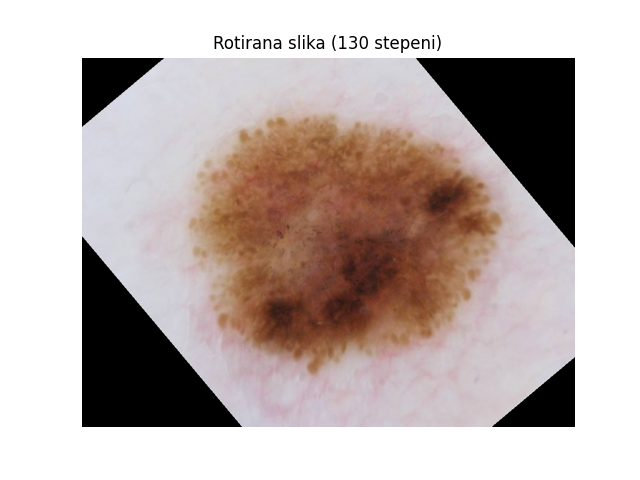
\includegraphics[width=0.3\textwidth]{slike_raka/rotated_image.png} 
        \caption{Prikaz rotirane instance za 45 stepeni} 
        \label{rotacija}
    \end{figure}
    \item Horizontalni obrt - simetrično slika piksele u odnosu na y osu
    \begin{figure}[H]
        \centering
        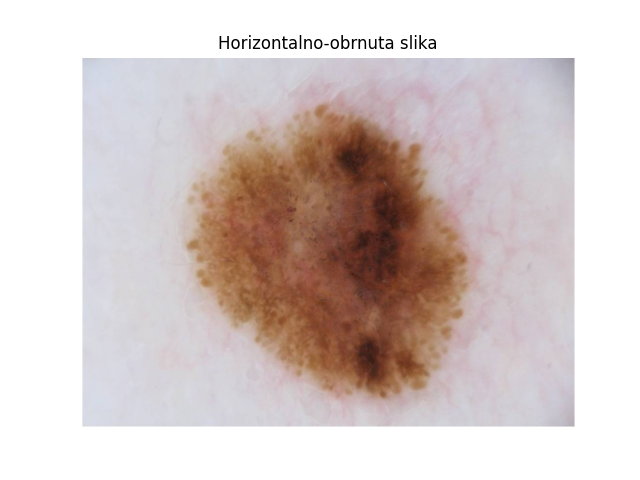
\includegraphics[width=0.3\textwidth]{slike_raka/horizontal_flip_image.png} 
        \caption{Prikaz horizontalno okrenute instance} 
        \label{horizontalno okrenuta instanca}
    \end{figure}
    \item Vertikalni obrt - simetrično slika piksele u odnosu na x osu
    \begin{figure}[H]
        \centering
        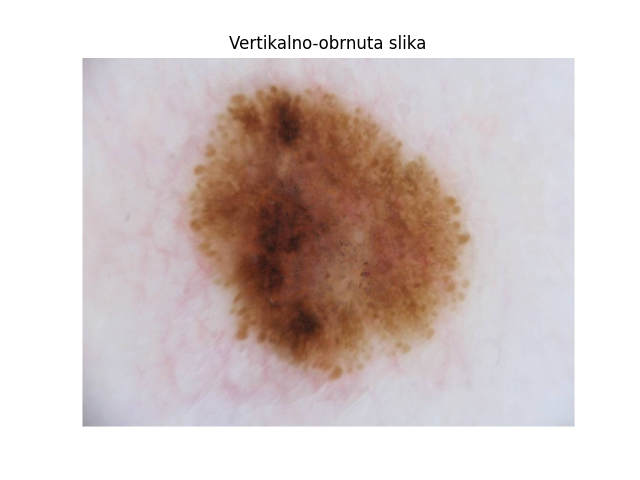
\includegraphics[width=0.3\textwidth]{slike_raka/vertical_flip_image.png} 
        \caption{Prikaz vertikalno okrenute instance} 
        \label{vertikalno okrenuta instanca}
    \end{figure}
\end{enumerate}
\par
Podaci se transformišu radi pretvaranja kategoričkih varijabli u numerički format, kao i inženjeerskih karakteristika radi kreiranja novih atributa ili izbora relevantnih atributa za analizu. Ovaj pristup ima posebnu primenu u radu sa XGBoost modelom s tim da on nije pogodan za primenu nad sirovim podacima slika već zahteva obradu skupa podataka kako bi mogao da se trenira.

\subsubsection{Validacioni skup}

Prilikom rada sa modelom koji koristi duboko mašinsko učenje, poželjno je pratiti njegov progres kroz trening epohe. Iz trening skupa, prilikom rada sa VGG modelom izdvojen je validacioni skup koji je uzeo prvih 10\% trening skupa iz svake klase pojedinačno. Ovo omogućava da se model evaluira posle svake epohe i da se prevremeno zaustavi ako bude bilo potrebe za tim zato što model koji se trenira na trening skupu, neće imati uvid u validacioni skup tokom treninga. Ako se desi skok funkcije gubitka na validacionom skupu, ovo može dati znak da se model preprilagođava, pa treba zaustaviti treniranje modela.

\subsection{Dodatni skup podataka za test - HAM10000}

Radi praćenja kvaliteta modela, dodata je podrška i za druge skupova podataka pri testiranju modela. To je demonstrirano dodavanjem HAM1000 [7] skupa koji sadrži 10015 slika, od kojih 1113 sadrži maligni tip raka, tj. 11.11\% celokupnog skupa podataka. Ostatak slika je obeležen kao benigni tip.

\section{Modeli}

Upotreba različitih modela za klasifikaciju je od velike koristi zbog razlike u arhitekturi modela i služi kao dobra metrika poređenja različitih metoda. Korišćena su dva različita modela za upoređivanje, jedan baziran na dubokim neuronskim mrežama i drugi na baziran na drvima odlučivanja.

\subsection{VGG}

\subsubsection{O modelu}

VGG (Visual Geometry Group) ima arhitekturu konvolucione neuronske mreže, razvijen je na Oksfordskom univerzitetu 2014. godine.
\par
VGG-11 je varijanta VGG-a sačinjena od 11 slojeva, uklučujući konvolucione, maksimalno-bazenske \textit{(eng. max-pooling)} i potpuno povezane slojeve [4]. Karakterističan je po tome što koristi male 3x3 konvolucione filtere sa pomerajem veličine 1 piksel i 2x2 maksimalno-bazenske slojeve sa pomerajem 2, što pomaže sa čuvanjem informacija i efikasno identifikuje složene uzorke u prostoru karakteristika slike, zadržavajucći razuman broj parametara unutar neuronske mreze. Model takođe sadrži i normalizaciju po grupama \textit{(eng. batch normalization)}

\begin{figure}[H]
    \centering
    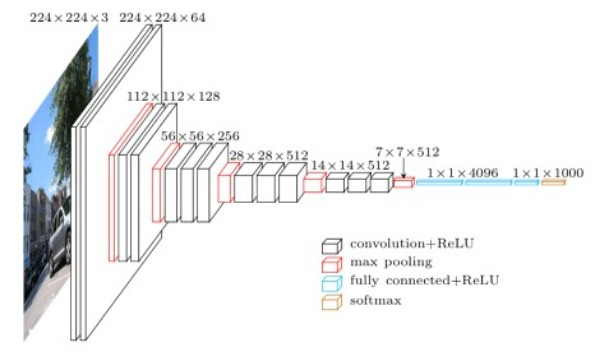
\includegraphics[width=0.8\textwidth]{vgg.jpg} 
    \caption{Prikaz arhitekture VGG-11} 
    \label{Arhitektura VGG11}
\end{figure}

Prednost VGG-11 modela je u tome što ne zahteva nikakvu vrstu izdvajanja karakteristika, već radi automatski nad sirovim podacima slika. Samim tim što je baziran na dubokim neuronskim mrežama, ima mogućnost da uoči kompleksne obrasce u reprezentaciji slike. Koriščen je pretreniran VGG model nad velikim skupom podataka ImageNet. Na ovaj način je model već naučen da prepoznaje mnoštvo detalja sa slika koje se kasnije mogu primeniti na naš skup podataka.

\subsubsection{Izlazna funkcija}
Izlazna funkcija je Softmax koja pretvara izlazne vrednosti iz neuronskih mreza u verovatnosnu vrednost za svaku od ciljnih klasa.
Matematička formula Softmax funkcije za vektor \(\mathbf{z}\) od \(n\) elemenata je:

\[ \sigma(\mathbf{z})_i = \frac{e^{z_i}}{\sum_{j=1}^n e^{z_j}} \]

Gde je:
\begin{itemize}
    \item \( \sigma(\mathbf{z})_i \) verovatnoća klase \(i\)
    \item \( z_i \) ulazna vrednost za klasu \(i\)
    \item \( n \) ukupan broj klasa
\end{itemize}

Ova funkcija osigurava da sve izlazne vrednosti budu nenegativne i da njihov zbir bude 1, što ih čini pogodnim za interpretaciju kao verovatnoće.

\subsubsection{Hiperparametri}

Hiperparametri su ključni za treniranje modela mašinskog učenja, jer određuju kako će model učiti iz podataka. Model u projektu koristi sledeće hiperparametre:

\begin{itemize}
    \item \textbf{Veličina grupe}: Veličina grupe \textit{(eng. Batch Size)} od 256 označava broj primera iz skupa podataka koji će se obraditi pre nego što se parametri modela ažuriraju. Veća veličina grupe može ubrzati treniranje, ali zahteva više memorije.
    \item \textbf{Broj epoha}: Model će imati 12 epoha, što znači da će se skup podataka za trening iskoristiti 12 puta. Svaka epoha omogućava modelu da bolje nauči obrasce u podacima.
    \item \textbf{Stopa učenja}: Stopa učenja \textit{(eng. Learning Rate)} je postavljena na $10^{-4}$, što određuje korak kojim se parametri modela ažuriraju tokom treniranja. Manja stopa učenja može dovesti do stabilnijeg konvergiranja, dok veća stopa može ubrzati učenje, ali i izazvati nestabilnost.
    \item \textbf{Korak stope učenja}: Korak stope učenja je 10, što znači da će se stopa učenja smanjivati svakih 10 epoha kako bi se omogućilo finije podešavanje modela tokom treniranja.
    \item \textbf{Funkcija gubitka}: Koristi se utežinjena unakrsna entropija kako bismo kompenzovali neravnotežu između klasa u skupu podataka. Ova funkcija meri razliku između predikcija modela i stvarnih vrednosti.
    \item \textbf{Optimizator}: Adam optimizator je odabran za treniranje modela. On kombinuje prednosti dva druga optimizatora, AdaGrad i RMSProp, i omogućava brže i efikasnije treniranje modela zahvaljujući adaptivnom koraku učenja za svaki parametar [6].
\end{itemize}

\subsection{XGBoost}

\subsubsection{O modelu}
XGBoost (Extreme Gradient Boosting) je metod mašinskog učenja zasnovan na drvetima odlučivanja [5]. Radi tako što gradi seriju drveća odlučivanja sekvencijalno, gde svako sledeće drvo ispravlja greške napravljene od strane prethodnih. Arhitektura XGBoost-a se sastoji od više drveća odlučivanja raspoređenih u ansamblu pojačavanja, pri čemu svako drvo uči da predviđa ostatke prethodnih drveća.
\begin{figure}[H]
    \centering
    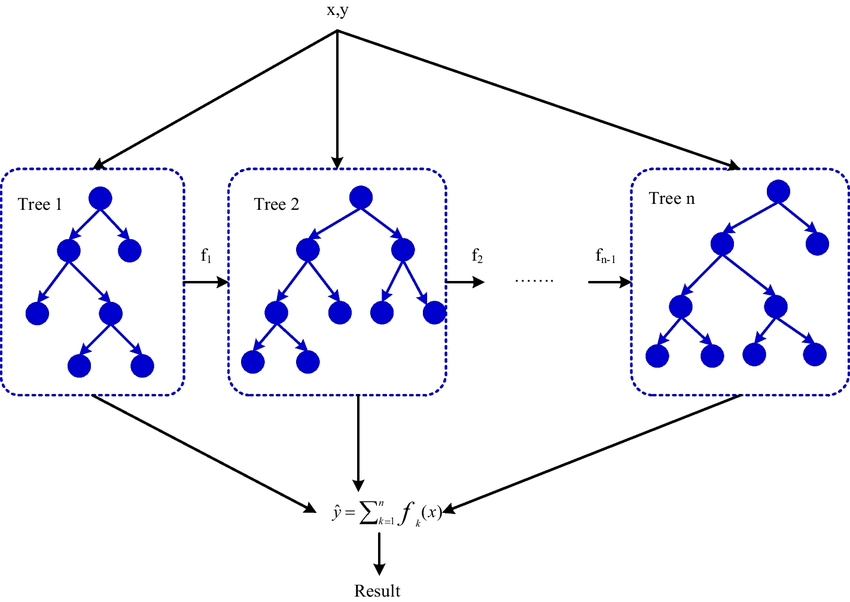
\includegraphics[width=0.5\textwidth]{xgboost.png} 
    \caption{Prikaz arhitekture XGBoost-a} 
    \label{arhitektura xgboost-a}
\end{figure}

XGBoost se tradicionalno koristi za klasifikaciju tabularnih podataka, pa je nužno izvršiti neku vrstu izdvajanja atributa. Ovo je urađeno tako što su ulazne spljošćene na jednodimenzione nizove, koju XGBoost prima za ulaz.

\subsubsection{Hiperparametri}

Koristeći GridSearchCV, klasu biblioteke \textit{scikit-learn}, otkriveni su najbolji hiperparametri za XGBoost model. Ovi hiperparametri su:

\begin{itemize}
    \item \textbf{Tip uzorkovanja}: Tip uzorkovanja \textit{(eng. sample type)} je postavljen na \textit{utežinjen} \textit{(eng. weighted)}, 
    što znači da se uzorci težinski ocenjuju tokom treniranja kako bi se poboljšala tačnost modela, posebno u slučajevima neravnoteže između klasa.
    \item \textbf{Stopa učenja}: Stopa učenja je postavljena na $10^{-2}$, što određuje korak kojim se parametri modela ažuriraju tokom treniranja.
    \item \textbf{Maksimalna dubina}: Maksimalna dubina stabla je 3, što ograničava broj nivoa u svakom odlučujućem stablu.
    \item \textbf{Broj procenitelja}: Postavljen je na 200, što znači da model koristi 200 odlučujućih stabala za pravljenje konačne predikcije. 
\end{itemize}

\section{Ocenjivanje kvaliteta modela}
\subsection{F1 mera}

Preciznost \textit{(eng. precision)} predstavlja sposobnost modela da ne označi negativan uzorak kao pozitivan, a odziv \textit{(eng. recall)} predstavlja sposobnost modela da pronađe sve pozitivne uzorke. F1 mera je karakteristična po tome što daje isti prioritet preciznosti i odzivu, samim tim se može prikazati harmonijskom sredinom ove dve bitne metrike evaluacije modela. 
\par
Ako označimo broj ispravno klasifikovanih pozitivnih primera kao $TP$, negativnih kao $TN$, broj negativnih primera pogrešno klasifikovanih kao pozitivni kao $FP$ i broj pozitivnih primera pogrešno klasifikovanih kao negativni kao $FN$ dobijamo sledeće jednačine:

\begin{equation}
\text{Preciznost} = \frac{\text{TP}}{\text{TP} + \text{FP}}
\end{equation}

\begin{equation}
\text{Odziv} = \frac{\text{TP}}{\text{TP} + \text{FN}}
\end{equation}

\begin{equation}
\text{F1 mera} = 2 \cdot \frac{\text{Preciznost} \cdot \text{Odziv}}{\text{Preciznost} + \text{Odziv}}
\end{equation}

Harmonijska sredina se koristi u izračunavanju F1 mere jer više kažnjava ekstremne vrednosti nego aritmetička sredina. Ovo je jako korisno s obzirom na podatak da disbalans klasa postoji u ISIC skupu podataka, pa tačnost nije idealna metrika jer se fokusira samo na $TP$. Radi diverzifikacije metrika, projekat podržava i radi sa drugim metodama takođe kao što su tačnost, preciznost i odziv.

\subsection{Matrica konfuzije}

Matrica konfuzije je ključan alat u evaluaciji performansi modela klasifikacije. On omogućava pregled rezultata klasifikacije kroz matricu koja prikazuje stvarne protiv predviđenih vrednosti za svaku klasu i time pruža detaljan uvid u performanse modela, omogućavajući da identifikujemo koje klase model dobro prepoznaje, a koje klase su problematične. Kao deo rezultata, prikazana je i matrica konfuzije za test skup.

\subsection{Grafički prikaz treninga}

Tokom treninga VGG modela, važno je pratiti različite metrike performansi kako bi se osiguralo da model uči pravilno i da se ne pojavljuju problemi poput preprilagođavanja ili potprilagođavanja. Metrike koje su praćene tokom treninga su:
\begin{itemize}
    \item Funkcija gubitka
    \item Tačnost
    \item Preciznost
    \item Odziv
    \item F1 mera
\end{itemize}

Prikaz ovih metrika tokom treninga omogućava nam da pratimo kako se model poboljšava i prilagođava, kao i da identifikujemo trenutke kada je potrebno zaustaviti trening ili promeniti hiperparametre kako bi se postigli optimalni rezultati.


\section{Rezultati}

\subsection{VGG}

\subsubsection{Trening}

Prilikom treniranja, primećuje se zastoj posle 10-te epohe u metrikama kao što je F1 mera. Pokazano je da i povećavanje broja epoha na 30 ne postiže bolje rezultate gledajući te metrike, ali i funkciju gubitka.

\begin{figure}[H]
    \centering
    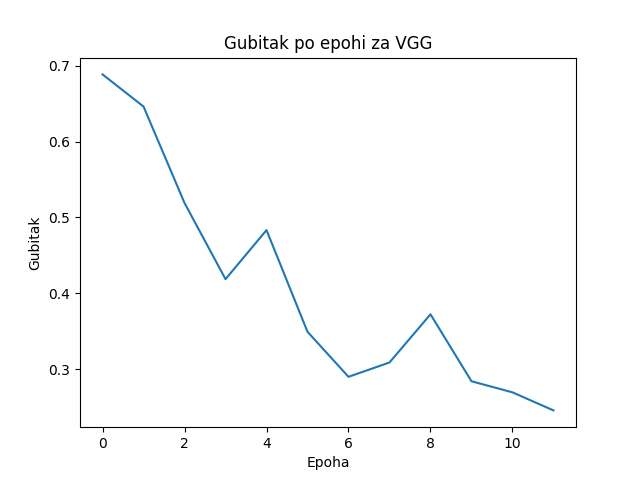
\includegraphics[width=0.6\textwidth]{rezultati/VGG_gubitak_po_epohi.png} 
    \caption{Funkcija gubitka kroz epohe za VGG-11 model} 
    \label{VGG gubitak po epohi}
\end{figure}

\begin{figure}[H]
    \centering
    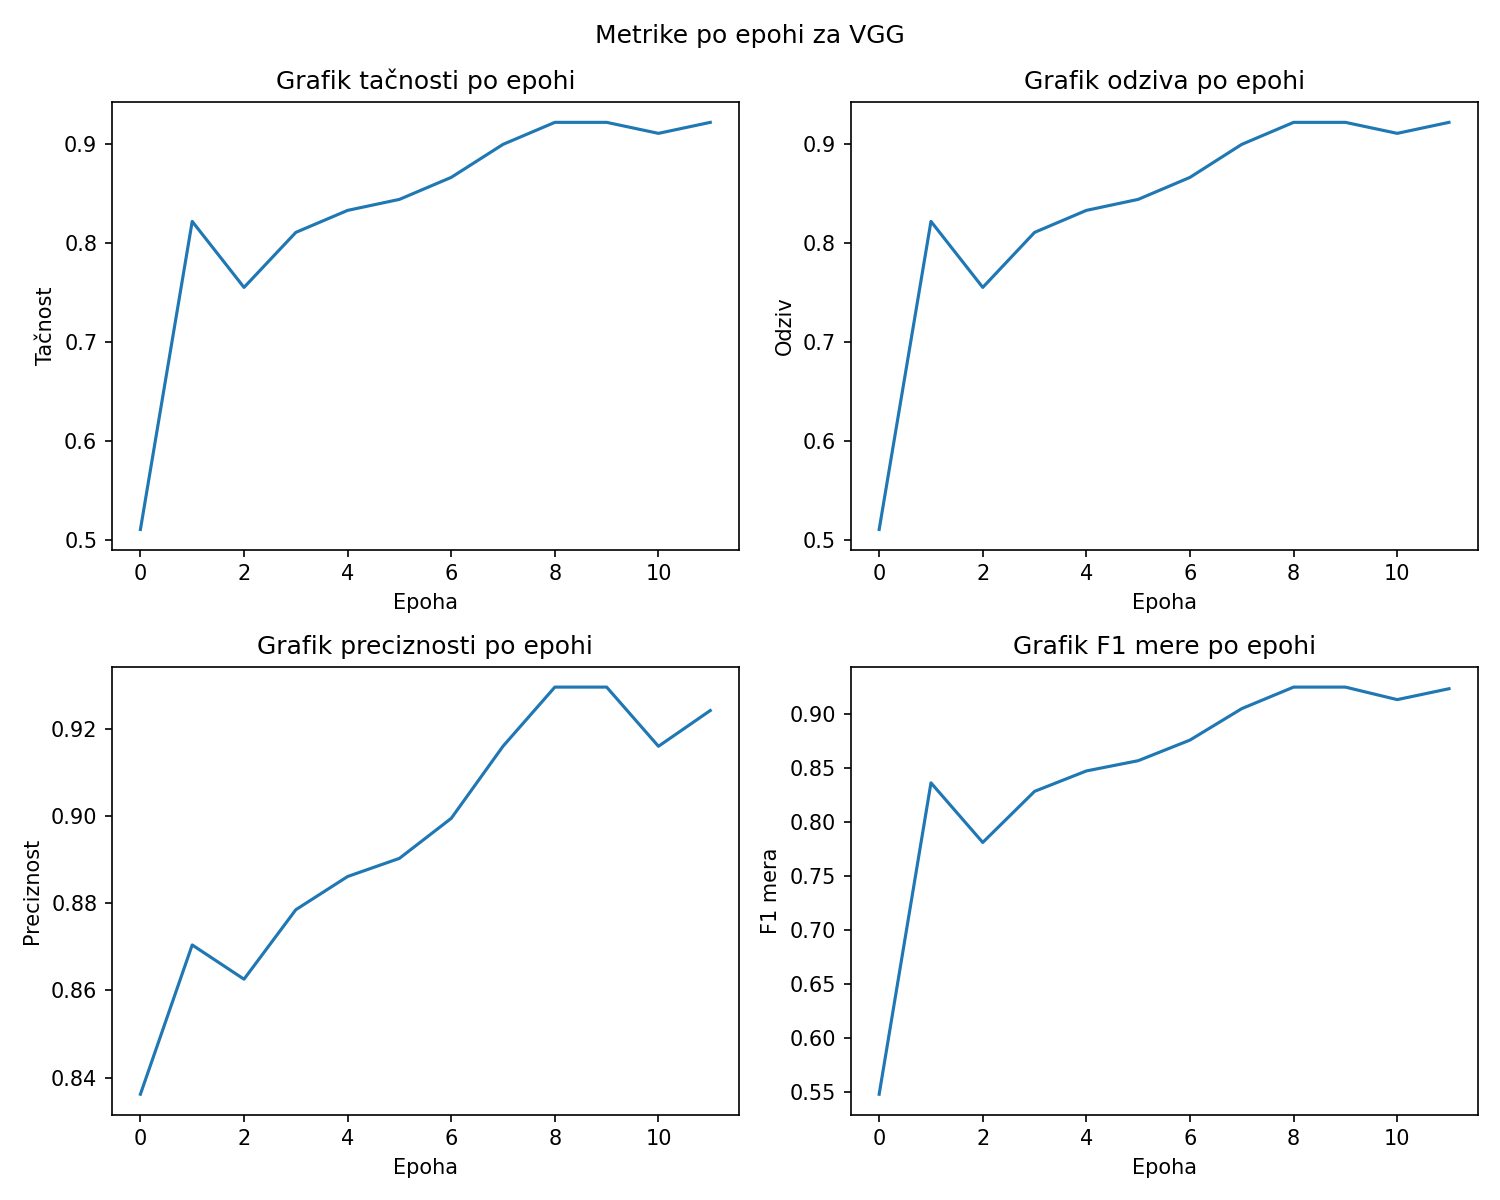
\includegraphics[width=0.8\textwidth]{rezultati/VGG_metrike_po_epohi.png} 
    \caption{Metrike kroz epohe za VGG-11 model} 
    \label{VGG metrike po epohi}
\end{figure}

\subsubsection{Test}

VGG-11 se pokazuje dobro, davajući rezultat 0.78 po F1 metrici. Vidi se da model uočava razlike između malignog i benignog raka, iako rezultati nisu savršeni.

\begin{figure}[H]
    \centering
    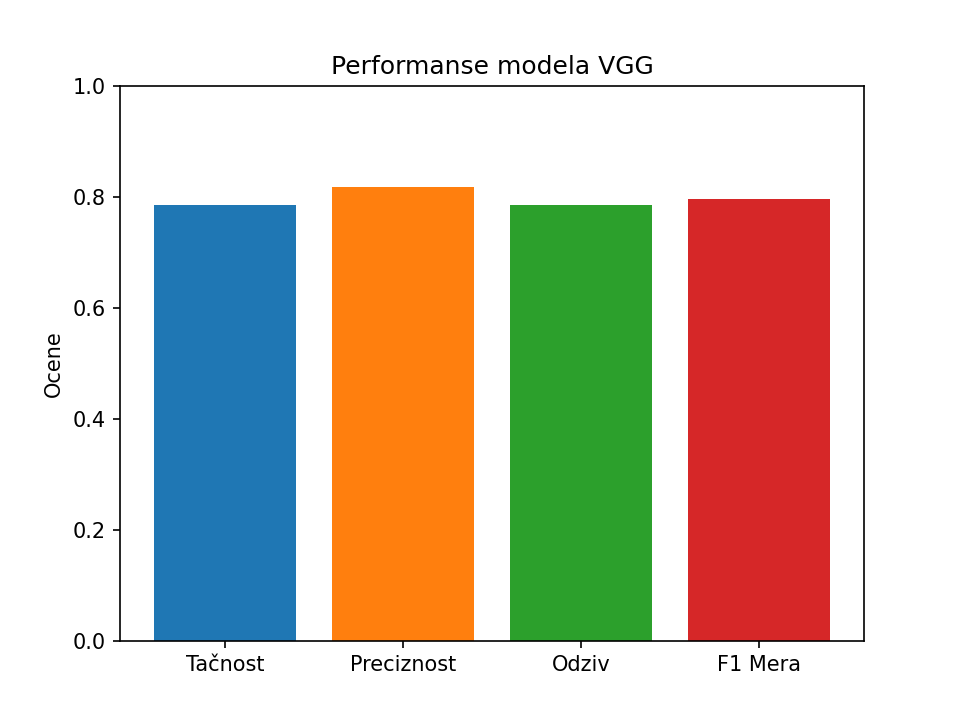
\includegraphics[width=0.5\textwidth]{rezultati/VGG_rezultati.png} 
    \caption{Rezultati za VGG-11 model} 
    \label{VGG rezultati}
\end{figure}

\begin{table}[H]
    \centering
    \begin{tabular}{|c|c|}
        \hline
        \textbf{Metrička vrednost} & \textbf{Rezultat} \\ \hline
        F1 mera & 0.80 \\ \hline
        Tačnost & 0.79 \\ \hline
        Preciznost & 0.82 \\ \hline
        Odziv & 0.79 \\ \hline
    \end{tabular}
    \caption{Tabela rezultate za VGG-11 model}
    \label{tab:vgg11_performance}
\end{table}

\begin{figure}[H]
    \centering
    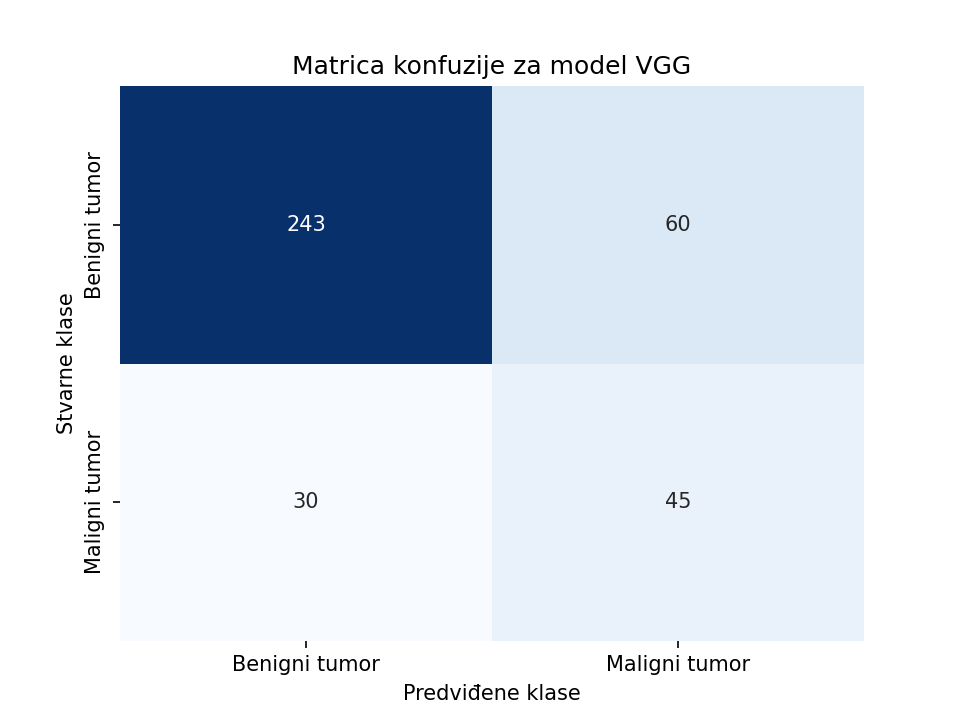
\includegraphics[width=0.7\textwidth]{rezultati/VGG_matrica_konfuzije.png} 
    \caption{Matrica konfuzije} 
    \label{VGG matrica konfuzije}
\end{figure}

Primećuje se jasna greška u predikciji malignog raka, kada je on zapravio bio benigni. Ovo pruža značajan uvid u greške modela i pretpostavlja se da je jedan od glavnih uzroka za ovo ponašanje mala količina podataka za trening.

\subsection{XGBoost}

XGBoost ima jednostavniji princip treninga, bez postojanja epoha, te imamo grafičke rezultate samo za test skup podataka.

\begin{figure}[H]
    \centering
    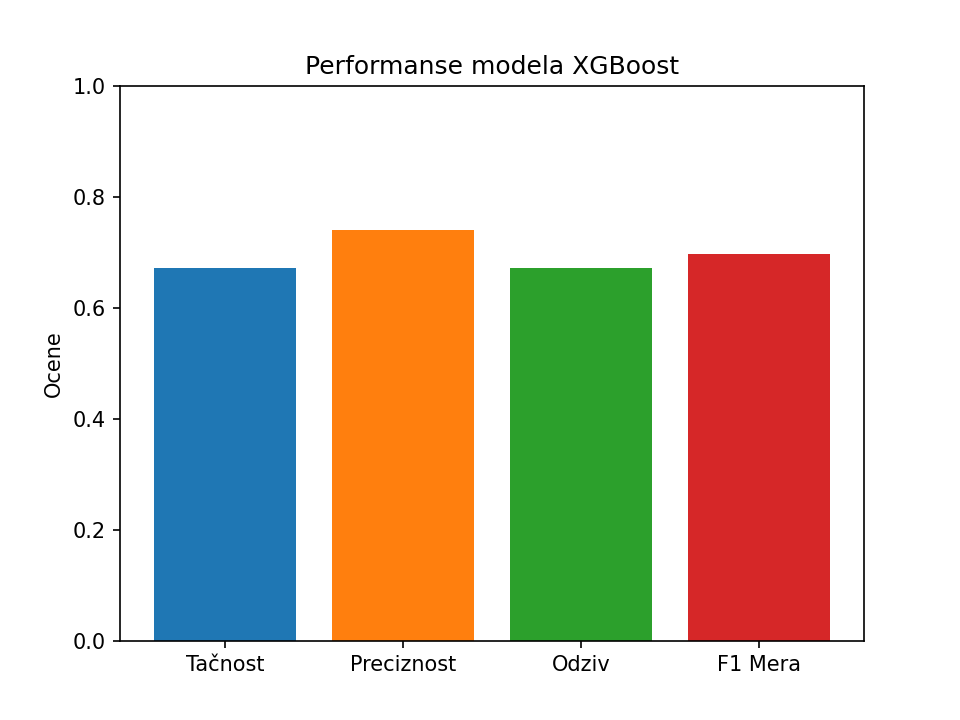
\includegraphics[width=0.5\textwidth]{rezultati/XGBoost_rezultati.png} 
    \caption{Rezultati za XGBoost model} 
    \label{XGBoost rezultati}
\end{figure}

\begin{table}[H]
    \centering
    \begin{tabular}{|c|c|}
        \hline
        \textbf{Metrička vrednost} & \textbf{Rezultat} \\ \hline
        F1 mera & 0.70 \\ \hline
        Tačnost & 0.67 \\ \hline
        Preciznost & 0.74 \\ \hline
        Odziv & 0.67 \\ \hline
    \end{tabular}
    \caption{Tabela rezultate za XGBoost model}
    \label{tab:XGBoost tabela rezultata}
\end{table}

\begin{figure}[H]
    \centering
    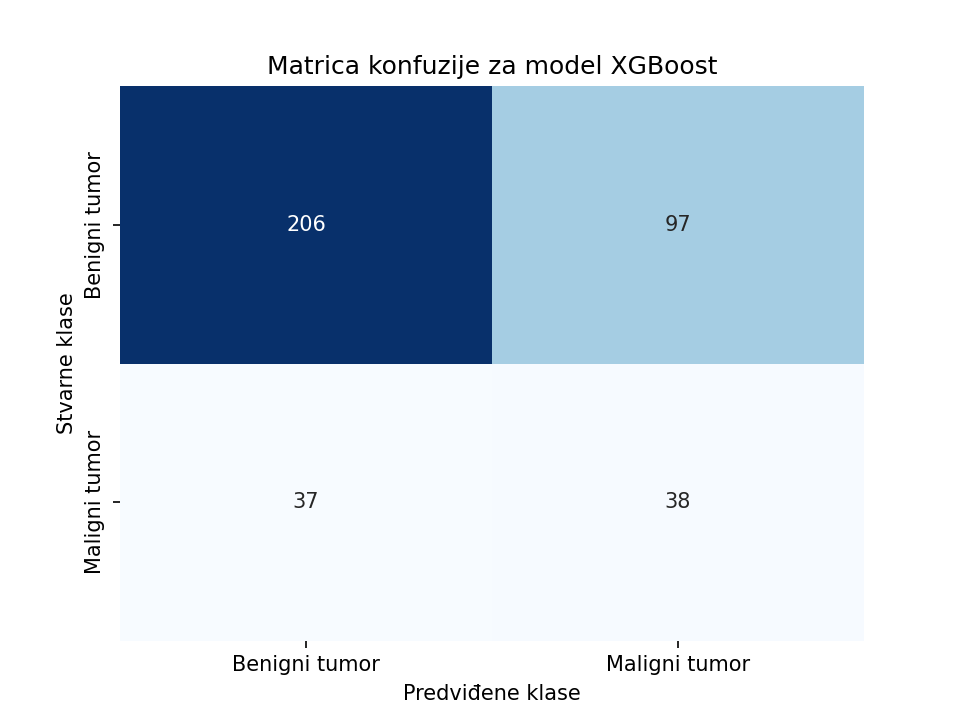
\includegraphics[width=0.7\textwidth]{rezultati/XGBoost_matrica_konfuzije.png} 
    \caption{XGBoost matrica konfuzije} 
    \label{XGBoost matrica konfuzije}
\end{figure}

Slično kao i kod VGG modela, XGBoost predviđa pogrešno relativno velik procenat benignog raka kao maligni. Pretpostavlja se da je glavni uzrok i ovde mala količina trening podataka.

\subsection{Poređenje}

VGG, iako sporiji u treningu, pokazuje se bolji u rezultatima po svakoj metrici. Ovakvi rezultati mogu da budu pripisani većoj moći za učenje modela VGG, koji se uspešnije pokazuje i u industriji za zadatke klasifikacije raznih pojmova u kompjuterskoj viziji.

\begin{table}[H]
\centering
\begin{tabular}{|c|c|c|}
\hline
\textbf{Metrička vrednost} & \textbf{XGBoost} & \textbf{VGG-11} \\ \hline
F1 mera & 0.70 & \textbf{0.80} \\ \hline
Tačnost & 0.67 & \textbf{0.79} \\ \hline
Preciznost & 0.74 & \textbf{0.82} \\ \hline
Odziv & 0.67 & \textbf{0.79} \\ \hline
\end{tabular}
\caption{Uporedni rezultati za XGBoost i VGG-11 modele}
\label{tab:comparison_performance}
\end{table}

\subsection{Test na HAM10000 skupu podataka}

Rezultati na ovom skupu potvrđuju gornje rezultate, davajući sličan rezultat po različitim metrikama. Gledajući F1 meru, VGG i ovde predstavlja bolji model, davajući 0.74 rezultat u poređenju sa XGBoost modelom koji daje rezultat 0.64.

\subsubsection{VGG}

\begin{table}[H]
    \centering
    \begin{tabular}{|c|c|}
        \hline
        \textbf{Metrička vrednost} & \textbf{Rezultat} \\ \hline
        F1 mera & 0.74 \\ \hline
        Tačnost & 0.68 \\ \hline
        Preciznost & 0.85 \\ \hline
        Odziv & 0.68 \\ \hline
    \end{tabular}
    \caption{Tabela rezultate za VGG-11 model na HAM skupu}
    \label{tab:xgboost_performance}
\end{table}

\begin{figure}[H]
    \centering
    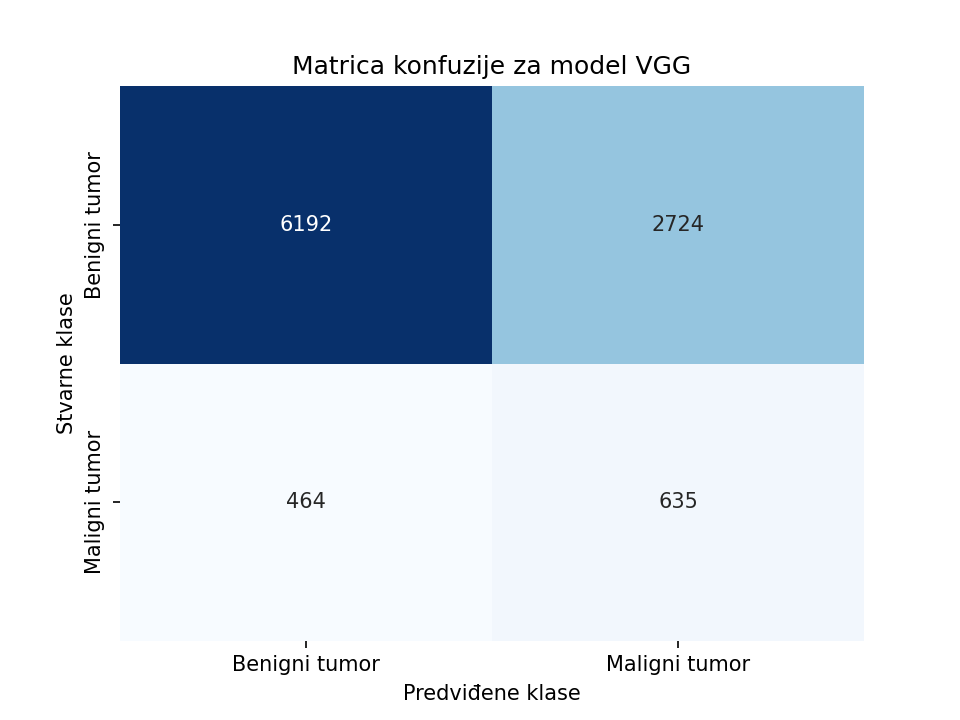
\includegraphics[width=0.7\textwidth]{rezultati/VGG_HAM_matrica_konfuzije.png} 
    \caption{VGG-11 matrica konfuzije na HAM skupu} 
    \label{VGG HAM matrica konfuzije}
\end{figure}

\subsubsection{XGBoost}
\begin{table}[H]
    \centering
    \begin{tabular}{|c|c|}
        \hline
        \textbf{Metrička vrednost} & \textbf{Rezultat} \\ \hline
        F1 mera & 0.68 \\ \hline
        Tačnost & 0.60 \\ \hline
        Preciznost & 0.83 \\ \hline
        Odziv & 0.60 \\ \hline
    \end{tabular}
    \caption{Tabela rezultate za XGBoost model na HAM skupu}
    \label{tab:XGbBoost rezultati na HAM skupu}
\end{table}

\begin{figure}[H]
    \centering
    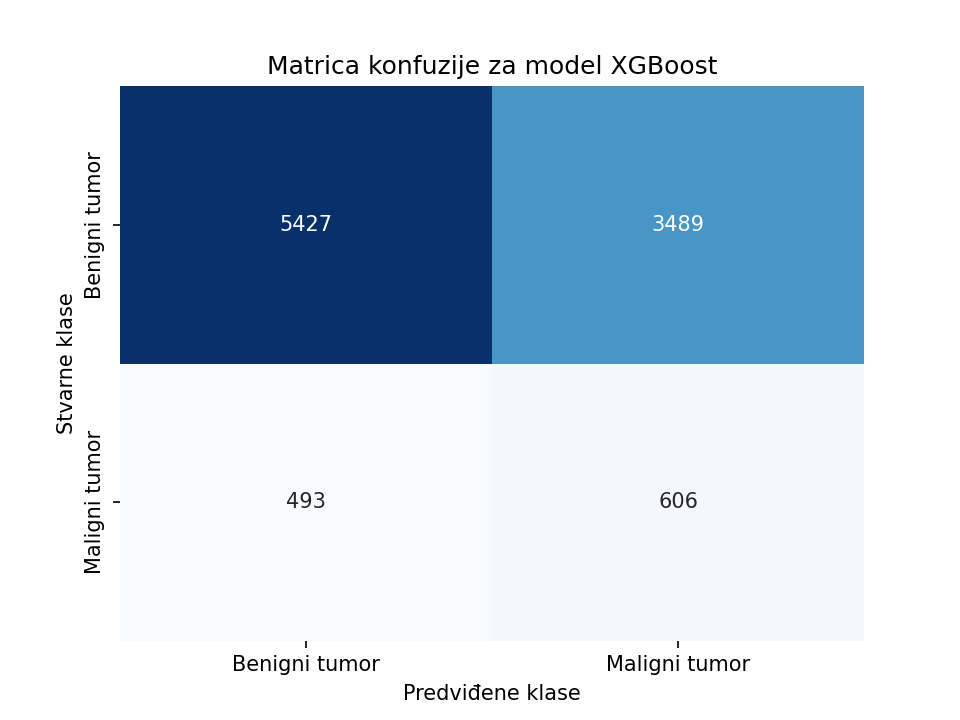
\includegraphics[width=0.7\textwidth]{rezultati/XGBoost_HAM_matrica_konfuzije.png} 
    \caption{XGBoost matrica konfuzije na HAM skupu} 
    \label{XGBoost HAM matrica konfuzije}
\end{figure}

\section{Zaključak}
Ovaj rad je produbio znanje autora o temama klasifikacije, i pokazao superiornost modela sa dubokim učenjem. Za dalji napredak ovog projekta, bio bi značajan veći i bolji skup podataka za trening, koji je izbegnut zbog ogromne veličine datoteka tj. manjka resursa.

\section{Literatura}

\begin{enumerate}[label={[\arabic*]}]
  \item Leiter, U.; Eigentler, T.; Garbe, C. Epidemiology of skin cancer. In Sunlight, Vitamin D and Skin Cancer; Springer: Berlin/Heidelberg, Germany, 2014; pp. 120–140.
  \item International Agency for Research on Cancer. Cancer—World Health Organization. 2020. Available online: https://www.who.int/cancer/PRGlobocanFinal.pdf (accessed on 15 December 2020).
  \item Ranpreet Kaur, Hamid GholamHosseini, Roopak Sinha and Maria Lindén, "Melanoma Classification Using a Novel Deep Convolutional Neural Network with Dermoscopic Images", Journal of Medical Imaging, 2020.
  \item K. Simonyan and A. Zisserman, “Very Deep Convolutional Networks for Large-Scale Image Recognition,” 2015. % VGG-11
  \item T. Chen and C. Guestrin, “XGBoost: A Scalable Tree Boosting System,” in Proceedings of the 22nd ACM SIGKDD International Conference on Knowledge Discovery and Data Mining, 2016. % XGBoost
  \item D. Kingma and J. Ba, “Adam: A Method for Stochastic Optimization,” 2014 
  \item P. Tschandl, C. Rosendahl, and H. Kittler, “The HAM10000 dataset, a large collection of multi-source dermatoscopic images of common pigmented skin lesions,” 2018.
  \item Gutman, D.; Codella, N. C. F.; Celebi, E.; Helba, B.; Marchetti, M.; Mishra, N.; Halpern, A., “Skin Lesion Analysis toward Melanoma Detection: A Challenge at the International Symposium on Biomedical Imaging (ISBI) 2016, hosted by the International Skin Imaging Collaboration (ISIC),” eprint arXiv:1605.01397, 2016.
  \item Van Rossum, G., \& Drake, F. L. The Python Language Reference, 2009.
  \item Paszke, A., Gross, S., Massa, F., Lerer, A., Bradbury, J., Chanan, G., … Chintala, S. (2019). PyTorch: An Imperative Style, High-Performance Deep Learning Library. In Advances in Neural Information Processing Systems 32 (pp. 8024–8035)
  \item Grbic, B.; Zolotarev, I. \href{https://github.com/Brankonymous/MelanomaClassification}{Github repositorium - Melanoma Classification}, 2024. 
\end{enumerate}

\end{document}
